\documentclass{beamer}

\usepackage[beamer]{shortcut}
\graphicspath{{./images/}}

\def\biblio{
    \nobibliography{library}
    \def\biblio{}
}

\institute{INRIA Saclay}
\author{Thomas Moreau}
\title{
    Curriculum learning
}

\setbeamertemplate{title page}[frame]
\def\extraLogo{}

\begin{document}

    \begin{frame}
        \titlepage
        \biblio{}
    \end{frame}

    \begin{frame}{Deep learning training with SGD}

        Training a deep model $f_\theta$:
       \[
            \min_\theta l(\theta) = \mathbb E \big[\mathcal L(y, f_\theta(X)) \big]
       \]

       \vskip2em
       {\centering \large Holistic algorithm: \textbf{Stochastic Gradient Descent}}
       \vskip2em
       \begin{enumerate}
        \item Sample a mini-batch of samples $\mathcal B$.
        \item Compute the gradient $\nabla_\theta l$
        \item Update the parameters $\theta -= \gamma\nabla_\theta l$.
       \end{enumerate}
       \vskip1em
       \strongpoint{How do you choose the mini-batch $\mathcal B$?}
    \end{frame}

    \frame{
        \frametitle{Curriculum Learning \mycite{Bengio2009}}

        Theory approach: random sampling\\[.5em]
        \small\qquad Take mini-batch at random, with replacement.\\[2em]

        Classic approach: random reshuffling\\[.5em]
        \small\qquad Take mini-batch at random, with replacement.\\[2em]

        Novel Idea: Curriculum learning\\[.5em]
        \small \qquad See easy samples first and increase the complexity as the training goes on.
    }

    \frame{
        \frametitle{Curriculum Learning}


        \begin{columns}
            \column{.5\textwidth}

            {\large $\Rightarrow$ Linked to continuation methods}\\[1em]
            \vskip2em

            {\large How to select easy/hard samples?}\\[1em]

            \begin{itemize}
                \item \textbf{Expert knowledge:} disagreement in annotation, domain knowledge, \dots
                \item \textbf{Difficulty proxy:} noise, sentence length, entropy, \dots
            \end{itemize}

            \column{.5\textwidth}
            \centering
            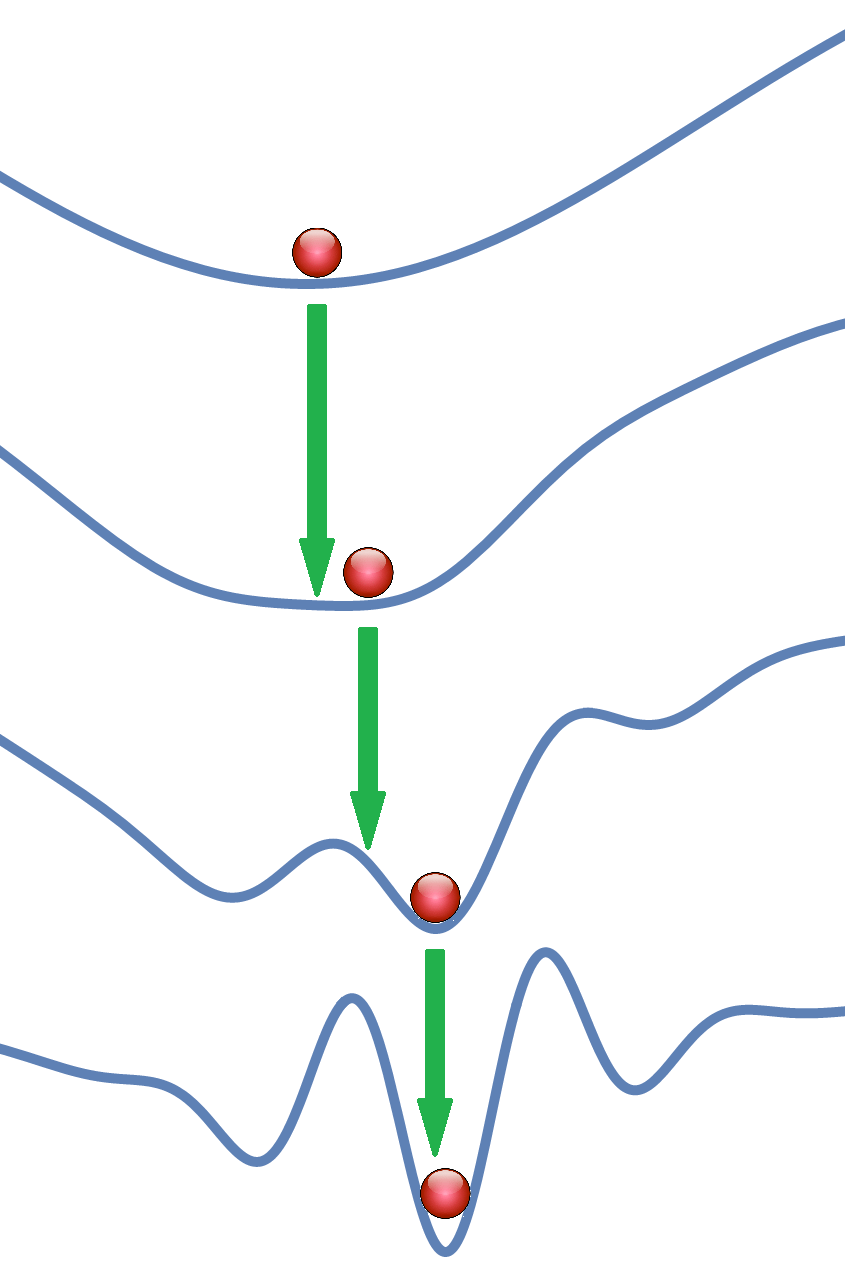
\includegraphics[width=.8\textwidth]{continuation_method}\\
        \end{columns}

    }

    \frame{
        \frametitle{Does it work?}

        Not so easy to find the answer!
        \vskip3em

        \strongpoint{We need to benchmark it!}

        \vskip2em\centering
        \includegraphics[width=.4\textwidth]{logo_benchopt}\\
    }

\end{document}